\documentclass{article}

% Language setting
% Replace `english' with e.g. `spanish' to change the document language
\usepackage[english]{babel}
\usepackage{amsmath}
\usepackage{algorithm}
\usepackage{algpseudocode}
\usepackage{tikz}

\usetikzlibrary{shapes.geometric, arrows, positioning}
\usepackage{geometry}
\geometry{margin=1in}

% Set page size and margins
% Replace `letterpaper' with `a4paper' for UK/EU standard size
\usepackage[letterpaper,top=2cm,bottom=2cm,left=3cm,right=3cm,marginparwidth=1.75cm]{geometry}

% Useful packages
\usepackage{amsmath}
\usepackage{graphicx}
\usepackage[colorlinks=true, allcolors=blue]{hyperref}
\usepackage{subcaption}

\title{Robot Foraging using Cluster Map CPFA \\ CSCI 8371 Swarm Robotics Final Project}
\author{Carlos Pena}
\date{December 2025}

\begin{document}

\maketitle

\section{Introduction}

The Central Place Foraging Algorithm (CPFA) is a bio-inspired swarm robotics algorithm based on the foraging behavior of desert harvester ants (\textit{Pogonomyrmex barbatus}) \cite{ants}. These ants efficiently locate and collect food resources in sparse, unpredictable environments by employing a combination of individual memory, pheromone trails, and probabilistic search strategies. The CPFA translates these biological mechanisms into a distributed algorithm that enables robot swarms to collectively forage without centralized control or direct inter-robot communication during search.

Traditional CPFA \cite{cpfa} implementations rely on three primary navigation modes: (1) site fidelity, where robots return to previously successful locations; (2) pheromone-guided search, where robots follow chemical trails laid by successful foragers; and (3) uninformed random search, where robots explore the arena without prior knowledge. While effective in many scenarios, standard CPFA exhibits limitations when resources are highly clustered or when certain regions remain unexplored due to stochastic search patterns.

\section{Motivation}

In realistic foraging scenarios, resources often exhibit spatial heterogeneity—some areas contain dense clusters of resources while others remain sparse. Standard CPFA, with its emphasis on exploiting known successful locations through site fidelity and pheromone reinforcement, can lead to incomplete exploration of the search space. Robots may repeatedly visit well-explored high-density regions while neglecting potentially resource-rich unexplored areas, resulting in suboptimal foraging efficiency.

This research addresses these limitations by introducing a Cluster-Mapping Enhanced CPFA (ClusterMap-CPFA), which augments the traditional algorithm with spatial awareness of exploration coverage. By maintaining a dynamic map of visited locations organized into hierarchical clusters, the enhanced system can identify underexplored regions and probabilistically direct search efforts toward them.

\section{Problem Definition}

The primary objective of this study is to compare the foraging performance of the traditional CPFA with the novel ClusterMap-CPFA approach. Specific research questions include:

\begin{enumerate}
    \item Does the addition of cluster-based exploration awareness improve overall foraging efficiency?
    \item How does the probability of searching low-cluster areas affect the balance between exploitation and exploration?
    \item Under what resource distribution scenarios (random, clustered, semi-clustered) does ClusterMap-CPFA demonstrate the most significant advantages?
    \item What is the computational overhead of maintaining and updating cluster maps in real-time?
\end{enumerate}

\section{Methods and Design}

Both algorithms were implemented and evaluated using the ARGoS (Autonomous Robots Go Swarming) multi-physics robot simulator \cite{argos}. The experimental setup consists of:

\subsection{Experimental Setup}

\begin{itemize}
    \item \textbf{Robot Platform:} FootBot agents with differential steering actuators and positioning sensors
    \item \textbf{Swarm Size:} 6 foraging robots per experiment
    \item \textbf{Arena Configuration:} 10m $\times$ 10m bounded environment with a central nest (0.25m radius)
    \item \textbf{Resources:} 256 food items total
    \item \textbf{Simulation Duration:} 30 minutes and 60 minutes per trial
    \item \textbf{Trials:} 10 independent runs per configuration for statistical validity
\end{itemize}

\subsection{Resource Distribution Scenarios}

Three distinct resource distribution patterns were implemented:

\begin{enumerate}
    \item \textbf{Random Distribution:} Resources uniformly distributed throughout the arena with no spatial correlation
    \item \textbf{Clustered Distribution:} Resources organized into 4 discrete clusters (8$\times$8 grid per cluster)
    \item \textbf{Semi-Clustered Distribution:} Power-law distribution creating clusters of varying sizes: 1$\times$1, 2$\times$2, 4$\times$4, and 8$\times$8, mimicking natural resource distributions
\end{enumerate}

\subsection{Standard CPFA Implementation}

The baseline CPFA implementation follows the established algorithm with the following behavioral parameters:

\begin{itemize}
    \item ProbabilityOfSwitchingToSearching = 0.504
    \item ProbabilityOfReturningToNest = 0.001
    \item UninformedSearchVariation = 7.0 degrees
    \item RateOfInformedSearchDecay = 0.28
    \item RateOfSiteFidelity = 4.27
    \item RateOfLayingPheromone = 3.75
    \item RateOfPheromoneDecay = 0.03
\end{itemize}

\subsubsection{Behavioral States}

\begin{figure}[h]
\centering
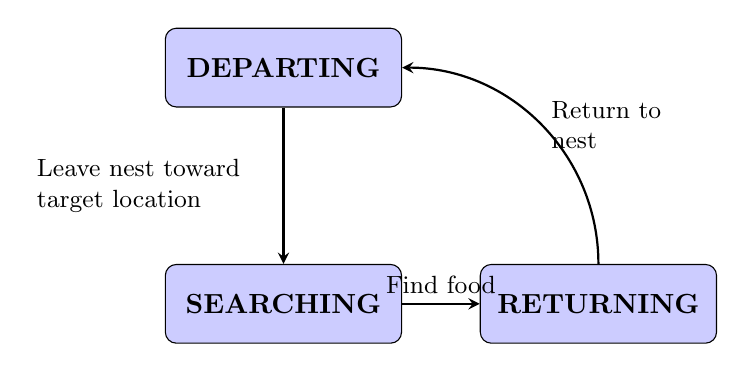
\begin{tikzpicture}[node distance=3cm, auto,
    state/.style={rectangle, rounded corners, minimum width=3cm, minimum height=1cm, 
                  text centered, draw=black, fill=blue!20, font=\bfseries},
    arrow/.style={->, >=stealth, thick}]
    
    % Nodes
    \node[state] (departing) {DEPARTING};
    \node[state, below of=departing] (searching) {SEARCHING};
    \node[state, right of=searching, node distance=4cm] (returning) {RETURNING};
    
    % Arrows
    \draw[arrow] (departing) -- node[left] {\parbox{3cm}{\small Leave nest toward\\target location}} (searching);
    \draw[arrow] (searching) -- node[above] {\parbox{3cm}{\centering\small Find food}} (returning);
    \draw[arrow] (returning.north) to[out=90, in=0] node[right] {\parbox{2cm}{\small Return to\\nest}} (departing.east);
    
\end{tikzpicture}
\caption{CPFA Behavioral State Diagram}
\end{figure}

\begin{description}
    \item[DEPARTING:] Robot leaves nest toward a target (random wall, pheromone waypoint, or site fidelity location)
    \item[SEARCHING:] Robot performs correlated random walk while monitoring for food
    \item[RETURNING:] Robot navigates back to nest with collected food
\end{description}

\subsubsection{Decision Hierarchy}

The CPFA decision hierarchy implements a three-tier priority system that determines the robot's next search strategy after successfully returning food to the nest. This hierarchical structure balances exploitation of known productive areas with exploration of new regions. At the highest priority, site fidelity allows robots to return to previously successful foraging locations, leveraging individual memory to exploit proven food sources. If site fidelity is not active or not selected probabilistically, the robot checks for pheromone trails laid by other agents, enabling indirect communication and collective learning about resource locations. When no informed search options are available, the robot defaults to uninformed search, randomly selecting a boundary point in the arena to promote exploration of unmapped areas. This decision structure ensures that robots progressively shift from exploration to exploitation as information accumulates in the system.

\begin{algorithm}[H]
\caption{CPFA Decision Hierarchy}
\begin{algorithmic}[1]
\If{site fidelity is active \textbf{and} probabilistically selected}
    \State Navigate to previous successful location
\ElsIf{pheromone trails exist}
    \State Follow strongest pheromone gradient
\Else
    \State Perform uninformed search toward random arena boundary
\EndIf
\end{algorithmic}
\end{algorithm}

\subsection{ClusterMap-CPFA Implementation}

The ClusterMap-CPFA extends the standard implementation with three key innovations:

\subsubsection{Spatial Memory and Visited Location Tracking}

Each robot maintains a local memory buffer of visited locations during foraging:

\begin{itemize}
    \item \textbf{Recording frequency:} Every 0.25 seconds during SEARCHING and DEPARTING states
    \item \textbf{Spatial tolerance:} 0.3m (prevents redundant recording of nearby points)
    \item \textbf{Storage limit:} 1000 locations per robot to prevent memory overflow
\end{itemize}

\subsubsection{Hierarchical Cluster Formation}

When a robot successfully returns to the nest with food, it shares its visited locations with a global map maintained by the loop functions. The system then performs hierarchical clustering:

\paragraph{Primary Clustering (Proximity-Based)}

The primary clustering algorithm processes the stream of visited locations shared by successful foraging robots to identify spatial concentrations of search activity. When a robot returns to the nest with food, its trajectory history is analyzed to form initial cluster representations. The algorithm iterates through each unassigned visited location and establishes it as a potential cluster center. All nearby points within a defined proximity threshold (40\% of the cluster radius) are then aggregated into this cluster, effectively grouping spatially coherent search activities. For each formed cluster, the algorithm calculates a centroid representing the geometric center of the visited points, determines the spatial bounds (minimum and maximum coordinates), and assigns a coverage metric based on point density. This coverage metric quantifies how thoroughly the cluster region has been explored, providing a foundation for subsequent search prioritization decisions. The proximity-based approach ensures that clusters capture meaningful spatial patterns in robot foraging behavior rather than isolated waypoints.

\begin{algorithm}[H]
\caption{Primary Clustering Algorithm}
\begin{algorithmic}[1]
\ForAll{unassigned visited locations}
    \State Create a new cluster centered at location
    \State Merge all nearby points within threshold (40\% of cluster radius)
    \State Calculate cluster centroid and bounds
    \State Assign coverage metric based on point density
\EndFor
\end{algorithmic}
\end{algorithm}

\paragraph{Secondary Clustering (Hierarchical Merging)}

The hierarchical merging algorithm refines the initial cluster set by identifying and combining overlapping or adjacent clusters into larger super-clusters. This iterative process prevents excessive fragmentation of the spatial representation while maintaining meaningful distinctions between distinct foraging regions. During each iteration, the algorithm evaluates all possible cluster pairs and calculates a combined area coverage ratio that measures the spatial relationship between clusters. When two clusters have a coverage ratio exceeding 40\%, indicating substantial overlap or proximity, they are merged into a single super-cluster. The original clusters are then deleted from the system, and a new merged cluster is created with updated bounds, centroid, and coverage metrics. This merging process continues iteratively until no further cluster pairs meet the merging criteria or until coverage converges to a stable configuration. The algorithm may terminate early if clusters expand to cover the entire arena, indicating comprehensive exploration. Importantly, merged clusters are flagged with an \texttt{isMerged} attribute, enabling differentiation between primary clusters (direct observations) and super-clusters (aggregated representations) for analysis and visualization purposes.

\begin{algorithm}[H]
\caption{Hierarchical Merging Algorithm}
\begin{algorithmic}[1]
\While{multiple clusters exist}
    \ForAll{cluster pairs}
        \State Calculate combined area coverage ratio
        \If{ratio $>$ 40\%}
            \State Merge clusters into super-cluster
            \State Delete original clusters, create new merged cluster
        \EndIf
    \EndFor
    \State Repeat until convergence or arena-wide coverage achieved
\EndWhile
\end{algorithmic}
\end{algorithm}

\paragraph{Key Properties}

\begin{itemize}
    \item Clusters are immutable after creation---they are never updated, only deleted and replaced during merging
    \item Prevents cluster ``drift'' that could confuse exploration targeting
    \item Merged clusters flagged with \texttt{isMerged = true} for visualization and analysis
\end{itemize}

\subsubsection{Low-Cluster Search Strategy}

A new search mode targets underexplored regions:

\paragraph{Grid-Based Coverage Analysis}
The grid-based coverage analysis algorithm identifies underexplored regions of the arena to guide robots toward areas with minimal search activity. The arena is discretized into a uniform $10 \times 10$ grid, creating 100 cells that serve as evaluation units for spatial coverage. For each grid cell, the algorithm calculates a total cluster influence score that quantifies how thoroughly that region has been explored. This influence calculation has two components: direct coverage, where cells completely within cluster bounds receive full influence, and distance-based decay, where nearby clusters contribute fractional influence that decreases with distance. This decay function ensures that cells adjacent to well-explored clusters receive partial coverage credit, preventing redundant searching in already-investigated neighborhoods. Cells with minimal total influence scores are identified as low-coverage regions and collected into a candidate set. The algorithm then randomly selects one cell from this set as the target for the next uninformed search, effectively balancing exploration of underexplored areas while maintaining stochastic variation in search patterns. This grid-based approach provides a computationally efficient method for identifying exploration gaps without requiring complex geometric calculations or path planning.

\begin{algorithm}[H]
\caption{Grid-Based Coverage Analysis}
\begin{algorithmic}[1]
\State Divide arena into $10 \times 10$ grid
\ForAll{grid cells}
    \State Calculate total cluster influence:
    \Indent
        \State Direct coverage (cell within cluster bounds)
        \State Distance-based decay (nearby clusters contribute fractionally)
    \EndIndent
    \State Track cells with minimal coverage
\EndFor
\State Select random cell from least-explored regions
\end{algorithmic}
\end{algorithm}

\paragraph{Integration into Decision Hierarchy}

The ClusterMap-CPFA enhanced decision hierarchy extends the standard CPFA decision structure by incorporating the low-cluster search strategy as an additional exploration mechanism. This modified hierarchy maintains the same high-level priority structure as standard CPFA, with site fidelity as the top priority and pheromone-following as the secondary option. However, when neither informed search strategy is available, the enhanced system introduces a probabilistic branch before defaulting to standard uninformed search. With a 30\% probability (governed by the \texttt{ProbabilityOfSearchingLowClusters} parameter), the robot activates the low-cluster search mode, targeting grid cells identified by the coverage analysis algorithm as underexplored regions. This targeted exploration helps robots discover resources in areas that have received minimal attention from the swarm. The remaining 70\% probability maintains standard uninformed search behavior, preserving the baseline exploration dynamics. This probabilistic integration ensures that the low-cluster search strategy supplements rather than replaces traditional exploration, allowing the system to balance targeted gap-filling with broad spatial coverage. The result is a hybrid approach that leverages collective spatial memory to improve exploration efficiency while maintaining the robustness and adaptability of the original CPFA algorithm.

\begin{algorithm}[H]
\caption{ClusterMap-CPFA Enhanced Decision Hierarchy}
\begin{algorithmic}[1]
\If{site fidelity is active \textbf{and} selected}
    \State Use site fidelity
\ElsIf{pheromone trails exist}
    \State Follow pheromones
\Else
    \State With probability ProbabilityOfSearchingLowClusters (30\%)
    \Indent
        \State Target low-cluster area
    \EndIndent
    \State Otherwise
    \Indent
        \State Perform standard uninformed search
    \EndIndent
\EndIf
\end{algorithmic}
\end{algorithm}

\begin{figure}[h]
\centering
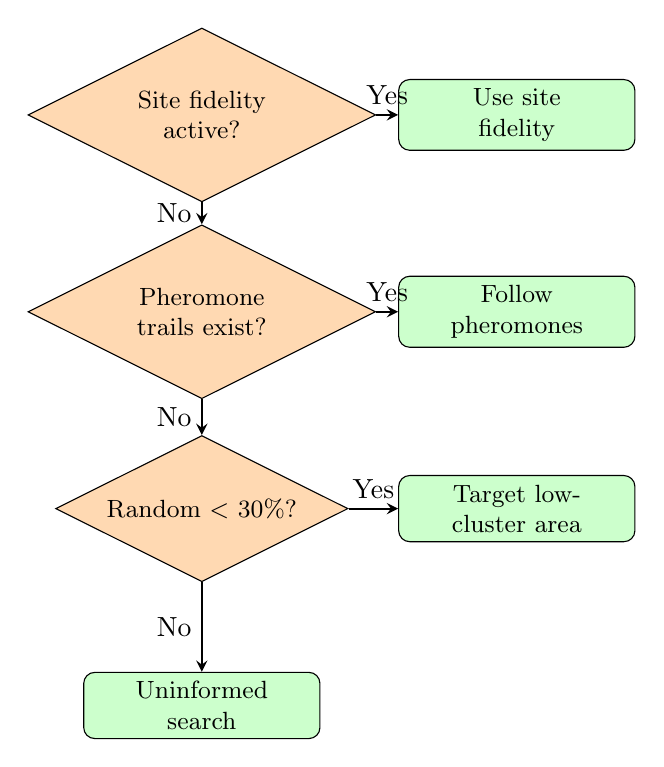
\begin{tikzpicture}[node distance=2.5cm, auto,
    decision/.style={diamond, aspect=2, minimum width=3cm, minimum height=1cm, 
                     text centered, draw=black, fill=orange!30, font=\small},
    action/.style={rectangle, rounded corners, minimum width=3cm, minimum height=0.8cm, 
                   text centered, draw=black, fill=green!20, font=\small},
    arrow/.style={->, >=stealth, thick}]
    
    % Nodes
    \node[decision] (sitefid) {\parbox{2.5cm}{\centering Site fidelity\\active?}};
    \node[action, right of=sitefid, node distance=4cm] (usesite) {\parbox{2.5cm}{\centering Use site\\fidelity}};
    \node[decision, below of=sitefid] (pheromone) {\parbox{2.5cm}{\centering Pheromone\\trails exist?}};
    \node[action, right of=pheromone, node distance=4cm] (followpher) {\parbox{2.5cm}{\centering Follow\\pheromones}};
    \node[decision, below of=pheromone] (lowcluster) {\parbox{2.5cm}{\centering Random $<$ 30\%?}};
    \node[action, right of=lowcluster, node distance=4cm] (targetlow) {\parbox{2.5cm}{\centering Target low-\\cluster area}};
    \node[action, below of=lowcluster] (uninformed) {\parbox{2.5cm}{\centering Uninformed\\search}};
    
    % Arrows
    \draw[arrow] (sitefid) -- node[above] {Yes} (usesite);
    \draw[arrow] (sitefid) -- node[left] {No} (pheromone);
    \draw[arrow] (pheromone) -- node[above] {Yes} (followpher);
    \draw[arrow] (pheromone) -- node[left] {No} (lowcluster);
    \draw[arrow] (lowcluster) -- node[above] {Yes} (targetlow);
    \draw[arrow] (lowcluster) -- node[left] {No} (uninformed);
    
\end{tikzpicture}
\caption{ClusterMap-CPFA Decision Flow Diagram}
\end{figure}

\begin{figure}[h]
\centering
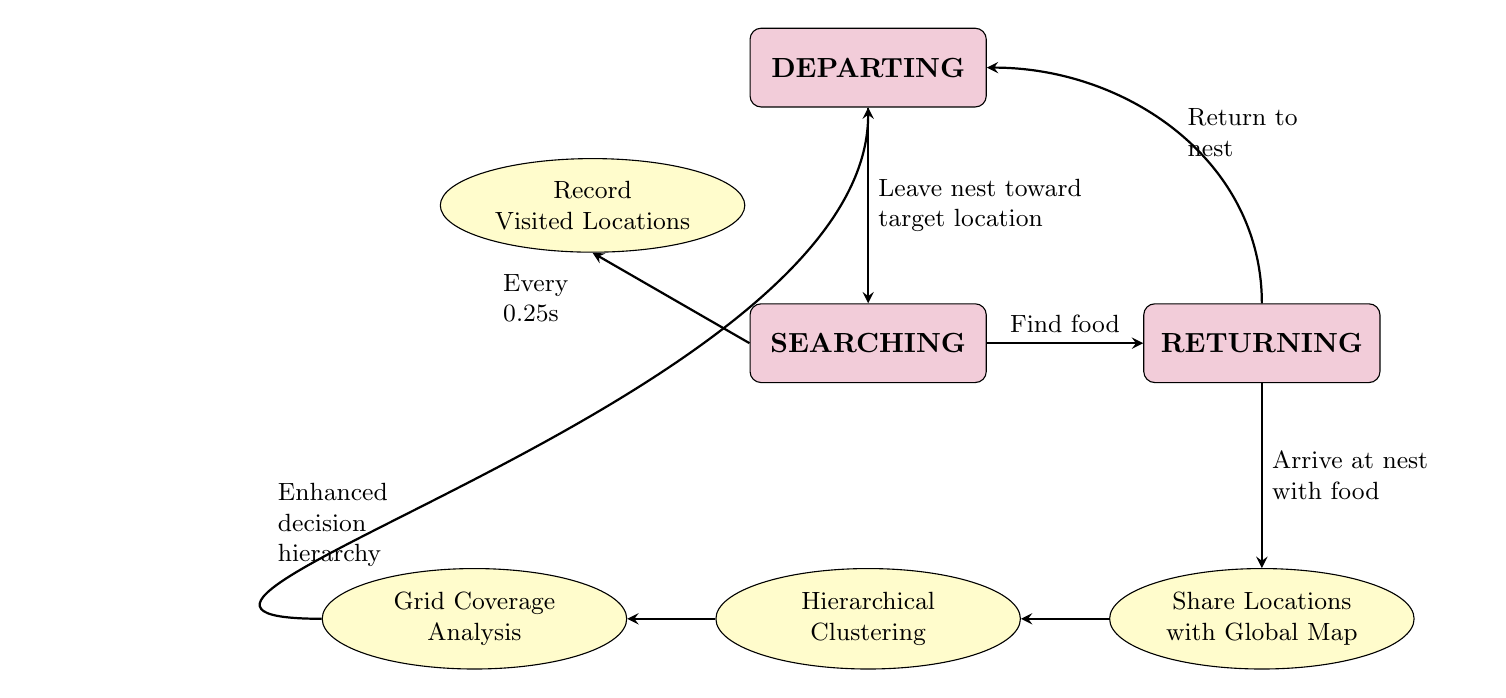
\begin{tikzpicture}[node distance=3.5cm, auto,
    state/.style={rectangle, rounded corners, minimum width=3cm, minimum height=1cm, 
                  text centered, draw=black, fill=purple!20, font=\bfseries},
    process/.style={ellipse, minimum width=2.5cm, minimum height=0.8cm,
                    text centered, draw=black, fill=yellow!20, font=\small},
    arrow/.style={->, >=stealth, thick}]
    
    % Nodes - centered layout
    \node[state] (departing) at (0,0) {DEPARTING};
    \node[process] (recording) at (-3.5,-1.75) {\parbox{2.5cm}{\centering Record\\Visited Locations}};
    \node[state] (searching) at (0,-3.5) {SEARCHING};
    \node[state] (returning) at (5,-3.5) {RETURNING};
    \node[process] (sharing) at (5,-7) {\parbox{2.5cm}{\centering Share Locations\\with Global Map}};
    \node[process] (clustering) at (0,-7) {\parbox{2.5cm}{\centering Hierarchical\\Clustering}};
    \node[process] (coverage) at (-5,-7) {\parbox{2.5cm}{\centering Grid Coverage\\Analysis}};
    
    % Arrows
    \draw[arrow] (departing) -- node[right] {\parbox{3.5cm}{\small Leave nest toward\\target location}} (searching);
    \draw[arrow] (searching) -- node[above] {\parbox{2.5cm}{\centering\small Find food}} (returning);
    \draw[arrow] (searching.west) -- node[left] {\parbox{2cm}{\small Every\\0.25s}} (recording.south);
    \draw[arrow] (returning) -- node[right] {\parbox{2.5cm}{\small Arrive at nest\\with food}} (sharing);
    \draw[arrow] (sharing) -- (clustering);
    \draw[arrow] (clustering) -- (coverage);
    \draw[arrow] (coverage.west) to[out=180, in=270] node[below left] {\parbox{2.5cm}{\small Enhanced\\decision\\hierarchy}} (departing.south);
    \draw[arrow] (returning.north) to[out=90, in=0] node[right] {\parbox{2cm}{\small Return to\\nest}} (departing.east);
    
\end{tikzpicture}
\caption{ClusterMap-CPFA Behavioral State Diagram with Memory and Clustering Integration}
\label{ClusterMap:states}
\end{figure}

\begin{description}
    \item[DEPARTING:] Robot leaves nest toward a target (random wall, pheromone waypoint, site fidelity location, or low-cluster area)
    \item[SEARCHING:] Robot performs correlated random walk while monitoring for food
    \item[RETURNING:] Robot navigates back to nest with collected food
    \item[Record Visited Locations:] Continuous process during DEPARTING and SEARCHING states (every 0.25s)
    \item[Share Locations with Global Map:] Upon successful food return, robot's trajectory history is uploaded
    \item[Hierarchical Clustering:] System performs primary clustering and hierarchical merging of visited locations
    \item[Grid Coverage Analysis:] System identifies underexplored regions for targeted exploration
\end{description}

\subsubsection{Visualization}

ClusterMap-CPFA provides enhanced visualization capabilities:

\begin{itemize}
    \item \textbf{Yellow dots:} Individual visited locations
    \item \textbf{Cyan squares:} Primary clusters (coverage $<$ 40\%)
    \item \textbf{Magenta squares:} Merged super-clusters (high coverage)
    \item \textbf{Real-time updates:} Clusters appear only after robot returns to nest
\end{itemize}

\begin{figure}[htbp]
    \centering
    \begin{subfigure}[t]{0.32\textwidth}
        \centering
        \includegraphics[width=\textwidth]{ClusterMap_siteVisited.png}
        \caption{Example view of robot path logging of visited locations. These are only shared and updated when the robot returns to the nest.}
        \label{fig:clusterMap_visited}
    \end{subfigure}
    \hfill
    \begin{subfigure}[t]{0.32\textwidth}
        \centering
        \includegraphics[width=\textwidth]{ClusterMap_siteVisited_clusters.png}
        \caption{Example view of how visited locations merge into a cluster when a threshold is achieved, typically when 40\% of the space is occupied within a 2 meter radius.}
        \label{fig:clusterMap_visited_to_cluster}
    \end{subfigure}
    \hfill
    \begin{subfigure}[t]{0.32\textwidth}
        \centering
        \includegraphics[width=\textwidth]{ClusterMap_clusters.png}
        \caption{Example of end state of the simulations when all visited locations have been merged into clusters.}
        \label{fig:clusterMap_final}
    \end{subfigure}
    \caption{Example of cluster formations in ARGoS showing progression from individual visited locations to merged clusters.}
    \label{fig:clusterMap_progression}
\end{figure}

\section{Results}

The experimental evaluation consisted of three distinct resource distribution scenarios, each executed with 10 independent simulation runs to ensure statistical validity. All experiments utilized a swarm of 6 foraging robots operating in an ARGoS environment. Both the standard CPFA and the proposed ClusterMap-CPFA algorithms were tested over durations of 30 minutes and 60 minutes under these conditions. Figure \ref{fig:distribution} shows the three different arena configurations used during the experiments. 

\begin{figure}[htbp]
    \centering
    \begin{subfigure}[b]{0.32\textwidth}
        \centering
        \includegraphics[width=\textwidth]{random_dist.png}
        \caption{Random distribution}
        \label{fig:random}
    \end{subfigure}
    \hfill
    \begin{subfigure}[b]{0.32\textwidth}
        \centering
        \includegraphics[width=\textwidth]{clustered_dist.png}
        \caption{Clustered distribution}
        \label{fig:clustered}
    \end{subfigure}
    \hfill
    \begin{subfigure}[b]{0.32\textwidth}
        \centering
        \includegraphics[width=\textwidth]{semi-dist.png}
        \caption{Semi-clustered distribution}
        \label{fig:semi-clustered}
    \end{subfigure}
    \caption{Three resource distribution scenarios used in experiments. (a) Resources randomly scattered throughout the arena, (b) All resources contained within 4 discrete clusters, (c) Power-law distributed clusters of varying sizes.}
    \label{fig:distribution}
\end{figure}

\subsection{Performance Metrics}

The primary performance metric was the number of resources successfully collected and returned to the nest within the allocated time period. Results are reported as mean $\pm$ standard deviation across 10 trials.



\subsection{30-Minute Trials}

\begin{table}[h]
\centering
\begin{tabular}{|l|c|c|c|}
\hline
\textbf{Distribution Type} & \textbf{CPFA} & \textbf{ClusterMap-CPFA} & \textbf{Improvement} \\
\hline
Random & $66.50 \pm 9.12$ & $86.80 \pm 3.46$ & +30.5\% \\
\hline
Semi-Clustered & $78.60 \pm 11.21$ & $86.50 \pm 5.36$ & +10.0\% \\
\hline
Clustered & $87.00 \pm 10.31$ & $69.30 \pm 4.60$ & $-$20.3\% \\
\hline
\end{tabular}
\caption{Resources collected (mean $\pm$ standard deviation) in 30-minute trials. ClusterMap-CPFA shows significant improvements in random and semi-clustered scenarios.}
\label{tab:algorithm_comparison_30min}
\end{table}

Table \ref{tab:algorithm_comparison_30min} presents the results of 30-minute experiments. In the random distribution scenario, ClusterMap-CPFA significantly outperforms CPFA by 30.5\% (86.80 vs. 66.50 resources), with substantially lower variance (3.46 vs. 9.12), indicating more consistent performance. This demonstrates that ClusterMap-CPFA is more effective at exploring the entire arena and locating scarce resources.

In the semi-clustered distribution, ClusterMap-CPFA shows a 10.0\% improvement over CPFA (86.50 vs. 78.60), with approximately half the variance. This demonstrates more consistent foraging in realistic scenarios where most resources are clustered, but many are scattered outside cluster boundaries.

In the clustered distribution, CPFA outperforms ClusterMap-CPFA by 20.3\% (87.00 vs. 69.30), suggesting that the traditional algorithm's site fidelity and pheromone mechanisms excel when resources are densely concentrated. However, we hypothesize that in natural environments, resources are rarely entirely contained within discrete clusters, making the semi-clustered distribution more ecologically realistic.

Overall, ClusterMap-CPFA consistently exhibits lower standard deviation across random and semi-clustered scenarios, indicating more predictable and stable foraging behavior.

\subsection{60-Minute Trials}

\begin{table}[h]
\centering
\begin{tabular}{|l|c|c|c|}
\hline
\textbf{Distribution Type} & \textbf{CPFA} & \textbf{ClusterMap-CPFA} & \textbf{Improvement} \\
\hline
Random & $125.20 \pm 10.76$ & $161.10 \pm 10.44$ & +28.7\% \\
\hline
Semi-Clustered & $158.60 \pm 12.76$ & $161.40 \pm 11.43$ & +1.8\% \\
\hline
Clustered & $170.40 \pm 13.11$ & $152.20 \pm 8.04$ & $-$10.7\% \\
\hline
\end{tabular}
\caption{Resources collected (mean $\pm$ standard deviation) in 60-minute trials. Extended duration narrows the performance gap in clustered scenarios.}
\label{tab:algorithm_comparison_60min}
\end{table}

Table \ref{tab:algorithm_comparison_60min} presents the results of 60-minute experiments. In the random distribution, ClusterMap-CPFA maintains its advantage, outperforming CPFA by 28.7\% (161.10 vs. 125.20), demonstrating sustained superior exploration capabilities.

In the semi-clustered distribution, both algorithms perform similarly (161.40 vs. 158.60), with ClusterMap-CPFA showing only a marginal 1.8\% advantage. This suggests that both strategies are equally effective in mixed spatial patterns when given sufficient time.

In the clustered distribution, CPFA outperforms ClusterMap-CPFA (170.40 vs. 152.20) by 10.7\%—a significantly reduced gap compared to the 30-minute trials. This indicates that ClusterMap-CPFA's exploration mechanisms eventually enable it to discover and exploit resource clusters, though at a slower initial rate than CPFA's site fidelity mechanism.

Notably, ClusterMap-CPFA shows lower standard deviation in the clustered condition (8.04 vs. 13.11), indicating more consistent performance, while both algorithms exhibit similar variability in random and semi-clustered conditions.

\section{Discussion and Conclusion}

The ClusterMap-CPFA algorithm demonstrates significant promise in addressing the challenge of foraging in environments with both clustered and sparse resource distributions. The experimental results reveal several key findings:

\subsection{Key Findings}

\begin{enumerate}
    \item \textbf{Superior Performance in Sparse Environments:} ClusterMap-CPFA consistently outperforms standard CPFA in random and semi-clustered scenarios, with improvements ranging from 10\% to 30\%. This advantage stems from the algorithm's ability to systematically identify and explore underexplored regions.
    
    \item \textbf{Improved Consistency:} ClusterMap-CPFA exhibits lower variance across most experimental conditions, indicating more reliable and predictable foraging behavior. This consistency is valuable for real-world deployments where performance predictability is critical.
    
    \item \textbf{Trade-offs in Dense Clustering:} In purely clustered environments, standard CPFA maintains an advantage during shorter time periods, suggesting that site fidelity and pheromone mechanisms are more efficient for exploiting known high-density resource patches. However, this gap narrows significantly over extended foraging periods.
    
    \item \textbf{Ecological Relevance:} The semi-clustered distribution, which mimics natural resource patterns, represents the most realistic scenario. In this condition, ClusterMap-CPFA demonstrates clear advantages, validating its utility for real-world applications.
\end{enumerate}

\subsection{Limitations and Future Work}

While ClusterMap-CPFA shows promising results, several limitations warrant further investigation:

\begin{itemize}
    \item \textbf{Computational Complexity:} The hierarchical clustering algorithm operates at O(n\textsuperscript{2}) complexity, making it computationally slower than standard CPFA. Future work should explore more efficient clustering methods, such as region-based neighbor-to-neighbor interactions, potentially reducing complexity to O(kn) where k is the number of regions and n is the number of clusters.
    
    \item \textbf{Parameter Sensitivity:} The algorithm's performance depends on several parameters (e.g., 30\% probability of low-cluster search, 40\% clustering threshold). Systematic parameter optimization through evolutionary algorithms or adaptive mechanisms could further improve performance.
    
    \item \textbf{Scalability:} Future experiments should evaluate performance with varying swarm sizes, arena dimensions, and resource densities to assess scalability.
    
    \item \textbf{Hardware Implementation:} Validation on physical robot platforms is necessary to assess real-world applicability, including challenges such as localization errors, communication constraints, and hardware limitations.
\end{itemize}

\subsection{Conclusion}

The ClusterMap-CPFA algorithm successfully extends the traditional CPFA framework by incorporating spatial awareness of exploration coverage. Through hierarchical clustering and targeted search strategies, the enhanced algorithm achieves superior performance in sparse and heterogeneous resource distributions while maintaining comparable efficiency in clustered environments. The increased consistency and reliability of ClusterMap-CPFA make it a valuable approach for swarm robotic foraging in complex, realistic environments. Future research should focus on computational optimization and hardware validation to enable practical deployment of this algorithm in real-world applications.

\section{References}

\bibliographystyle{abbrv}
\begin{thebibliography}{99}

\bibitem{ants}
Gordon, D. M. (1995). The development of an ant colony's foraging range. \textit{Animal Behaviour}, 49(3), 649-659.

\bibitem{cpfa}
Hecker, J. P., \& Moses, M. E. (2015). Beyond pheromones: evolving error-tolerant, flexible, and scalable ant-inspired robot swarms. \textit{Swarm Intelligence}, 9(1), 43-70.

\bibitem{argos}
Pinciroli, C., Trianni, V., O'Grady, R., Pini, G., Brutschy, A., Brambilla, M., ... \& Dorigo, M. (2012). ARGoS: a modular, parallel, multi-engine simulator for multi-robot systems. \textit{Swarm Intelligence}, 6(4), 271-295.

\end{thebibliography}

\end{document}
